\documentclass{prova}

\usepackage{amssymb}
\usepackage[inline]{enumitem}

\newcommand{\sen}{\,\mbox{sen}\,}
\newcommand{\tg}{\,\mbox{tg}\,}
\newcommand{\cosec}{\,\mbox{cosec}\,}
\newcommand{\cotg}{\,\mbox{cotg}\,}
\newcommand{\tr}{\,\mbox{tr}\,}
\newcommand{\ds}{\displaystyle}
\newcommand{\ra}{\rightarrow}

\professor{Prof.\@ Adriano Barbosa}
\disciplina{C\'alculo Diferencial e Integral}
\avaliacao{PS}
\curso{Eng.\@ de Alimentos}
\data{26/07/2018}

\begin{document}
	\cabecalho{5}  % o numero 5 indica a qnt de quadros na tabela de nota

	\textbf{Todas as respostas devem ser justificadas.}
    \vspace{0.5cm}

    {\bf Avalia\c{c}\~ao P1:}
	\begin{questionario}
        \q{Calcule os limites:}
            \begin{questionario}
                \qq{$\ds\lim_{x\ra25} \frac{x-25}{\sqrt{x}-5}$}
                \qq{$\ds\lim_{x\ra0} \frac{1-\sqrt{1-x^2}}{x}$}
            \end{questionario}
        \q{Determine o maior dom\'{i}nio de $\ds f(x) = \frac{x}{2x^2+x}$ e os
            valores de $x$ para os quais $f$ \'e cont\'{\i}nua.}
        \q{Calcule a derivada das fun\c{c}\~oes abaixo:}
            \begin{questionario}
                \qq{$\ds f(x) = \frac{x^2-x+2}{\sqrt{x}}$}
                \qq{$\ds f(x) = x^2\sen{(2x)}$}
            \end{questionario}
        \q{Dada $y=\sen{(\cos{(1+x^3)})}$. Calcule $\ds \frac{dy}{dx}$.}
        \q{Use deriva\c{c}\~ao impl\'{\i}cita para calcular $\ds \frac{dy}{dx}$, onde
            $y\cos{x}=x^2+y^2$.}
	\end{questionario}

    \vspace{1cm}

    {\bf Avalia\c{c}\~ao P2:}
    \begin{questionario}
        \q{Dois carros come\c{c}am a se mover a partir de um mesmo ponto. O
            primeiro viaja para sul a 60km/h e o segundo para oeste a 25km/h. A
            qual taxa a dist\^ancia entre os carros est\'a aumentando ap\'os duas
            horas da partida?}
        \q{Uma lata cil\'{\i}ndrica sem tampa deve comportar $1000$ cm$^3$ de
            l\'{\i}quido. Encontre as dimens\~oes que minimizam o custo do metal usado
            para fabricar a lata.}
        \q{Determine a fun\c{c}\~ao $f$ tal que $f'(x)=x^{-1/3}$, $f(1)=1$.}
        \q{Calcule a integral $\ds\int_1^9 \frac{\sqrt{u}-2u^2}{u}\ du$.}
        \q{O gr\'afico de $f$ \'e dado na figura abaixo. Calcule as integrais
            definidas:}
        \begin{figure}[h]
            \centering
            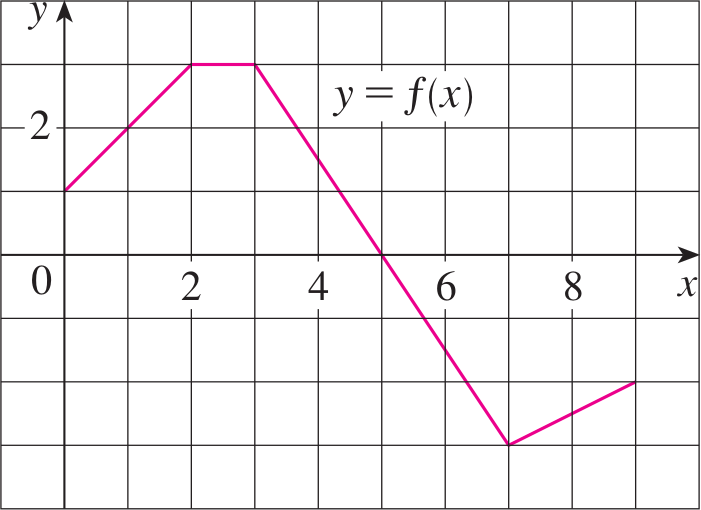
\includegraphics[width=0.4\textwidth]{area.png}
        \end{figure}

        \begin{enumerate*}
            \item $\ds\int_0^2 f(x)\ dx$
            \hspace{0.5cm}
            \hspace{0.5cm}
            \item $\ds\int_3^7 f(x)\ dx$
        \end{enumerate*}
    \end{questionario}
\end{document}
